\documentclass[a4paper,11pt,openany]{book}
\usepackage[T1]{fontenc}
\usepackage[utf8]{inputenc}
\usepackage{lmodern,hyperref,graphicx,tcolorbox,listings,fancyhdr,longtable,caption,color,dblfnote}
\usepackage[titletoc]{appendix}
\usepackage[english]{babel}

\tcbuselibrary{breakable}

\DFNalwaysdouble

\pagestyle{fancy}
\fancyhead[C]{FOT Developer's Manual}
\fancyhead[LE]{}
\fancyhead[RO]{}
\fancyhead[RE]{}
\fancyhead[LO]{}
\cfoot{\thepage}

%\newenvironment{dedication}
%{
%   \cleardoublepage
%   \thispagestyle{empty}
%   \vspace*{\stretch{1}}
%   \hfill\begin{minipage}[t]{0.66\textwidth}
%   \raggedright
%}
%{
%   \end{minipage}
%   \vspace*{\stretch{3}}
%   \clearpage
%}

%%%%%%%%%%%%%%%%%%%%%%%%%%%%%%%%%%%%%%%%%%%%%%%%
% Chapter quote at the start of chapter        %
% Source: http://tex.stackexchange.com/a/53380 %
%%%%%%%%%%%%%%%%%%%%%%%%%%%%%%%%%%%%%%%%%%%%%%%%
\lstset{
showstringspaces=false,
breaklines=true,
breakatwhitespace=false,
tabsize=3,
basicstyle=\ttfamily\footnotesize\linespread{0.2},
commentstyle=\color{red},
keywordstyle=\color{blue}
}
\newcommand{\urlthis}[2]{#2\footnote{#1}}
\makeatletter
\renewcommand{\@chapapp}{}% Not necessary...

%\newenvironment{chapquote}[2][2em]
%  {\setlength{\@tempdima}{#1}%
%   \def\chapquote@author{#2}%
%   \parshape 1 \@tempdima \dimexpr\textwidth-2\@tempdima\relax%
%   \itshape}
%  {\par\normalfont\hfill--\ \chapquote@author\hspace*{\@tempdima}\par\bigskip}
%\makeatother

%%%%%%%%%%%%%%%%%%%%%%%%%%%%%%%%%%%%%%%%%%%%%%%%%%%
% First page of book which contains 'stuff' like: %
%  - Book title, subtitle                         %
%  - Book author name                             %
%%%%%%%%%%%%%%%%%%%%%%%%%%%%%%%%%%%%%%%%%%%%%%%%%%%

% Book's title and subtitle
\title{\Huge \textbf{FOSSEE Optimization Toolbox}  %\footnote{This is a footnote.} 
\\ \huge Developer's Manual} %\footnote{April, 2017.}
% Author
\author{\href{mailto:toolbox@scilab.in}{toolbox@scilab.in}}%\thanks{\url{www.example.com}}}


\begin{document}

\frontmatter
\maketitle

%%%%%%%%%%%%%%%%%%%%%%%%%%%%%%%%%%%%%%%%%%%%%%%%%%%%%%%%%%%%%%%%
%% Add a dedication paragraph to dedicate your book to someone %
%%%%%%%%%%%%%%%%%%%%%%%%%%%%%%%%%%%%%%%%%%%%%%%%%%%%%%%%%%%%%%%%
%\begin{dedication}
%Dedicated to Calvin and Hobbes.
%\end{dedication}

%%%%%%%%%%%%%%%%%%%%%%%%%%%%%%%%%%%%%%%%%%%%%%%%%%%%%%%%%%%%%%%%%%%%%%%%
% Auto-generated table of contents, list of figures and list of tables %
%%%%%%%%%%%%%%%%%%%%%%%%%%%%%%%%%%%%%%%%%%%%%%%%%%%%%%%%%%%%%%%%%%%%%%%%
\tableofcontents
%\listoffigures
%\listoftables

\mainmatter

%%%%%%%%%%%
% Preface %
%%%%%%%%%%%
%\chapter*{Preface}
%Lorem ipsum dolor sit amet, consectetur adipiscing elit. Duis risus ante, auctor et pulvinar non, posuere ac lacus. Praesent egestas nisi id metus rhoncus ac lobortis sem hendrerit. Etiam et sapien eget lectus interdum posuere sit amet ac urna.
%
%\section*{Un-numbered sample section}
%Lorem ipsum dolor sit amet, consectetur adipiscing elit. Duis risus ante, auctor et pulvinar non, posuere ac lacus. Praesent egestas nisi id metus rhoncus ac lobortis sem hendrerit. Etiam et sapien eget lectus interdum posuere sit amet ac urna. Aliquam pellentesque imperdiet erat, eget consectetur felis malesuada quis. Pellentesque sollicitudin, odio sed dapibus eleifend, magna sem luctus turpis.
%
%\section*{Another sample section}
%Lorem ipsum dolor sit amet, consectetur adipiscing elit. Duis risus ante, auctor et pulvinar non, posuere ac lacus. Praesent egestas nisi id metus rhoncus ac lobortis sem hendrerit. Etiam et sapien eget lectus interdum posuere sit amet ac urna. Aliquam pellentesque imperdiet erat, eget consectetur felis malesuada quis. Pellentesque sollicitudin, odio sed dapibus eleifend, magna sem luctus turpis, id aliquam felis dolor eu diam. Etiam ullamcorper, nunc a accumsan adipiscing, turpis odio bibendum erat, id convallis magna eros nec metus.
%
%\section*{Structure of book}
%% You might want to add short description about each chapter in this book.
%Each unit will focus on <SOMETHING>.
%
%
%%%%%%%%%%%%%%%%%%%%%%%%%%%%%%%%%%%%%
%% Give credit where credit is due. %
%% Say thanks!                      %
%%%%%%%%%%%%%%%%%%%%%%%%%%%%%%%%%%%%%
%\section*{Acknowledgements}
%\begin{itemize}
%\item Lorem ipsum dolor sit amet, 
%\item Lorem ipsum dolor sit amet, 
%\end{itemize}
%\mbox{}\\
%%\mbox{}\\
%\noindent Google \\
%\noindent \url{http://google.com/}

%
%%%%%%%%%%%%%%%%%
%% NEW CHAPTER! %
%%%%%%%%%%%%%%%%%
\chapter{Introduction}

%\section{Section heading}
FOSSEE Optimization toolbox is a toolbox in Scilab maintained and developed by \urlthis{https://fossee.in/}{FOSSEE}(Free and Open Source Software in Education), \urlthis{http://iitb.ac.in/}{IIT Bombay}. It can solve the following optimization problems :

1. Linear programming(LP)

2. Quadratic programming(QP)

3. Nonlinear programming(NLP)

4. Integer programming(IP)

5. Second order Conic Programming(SOCP) problems

\noindent It also solves specific optimization problems like least squares, minimax and goal attainment problem.\\
Scilab is a open-source numerical computational package licensed under GPLv2 license which has broad applications in educational and engineering domains. It is a competitive alternative to Matlab and Octave. Scilab was initially maintained and developed by \urlthis{https://www.inria.fr/en/}{INRIA}(French Institute for Research in Computer Science and Automation). Scilab consortium was formed in June 2010 which now handles Scilab development.
FOSSEE Optimization toolbox uses a dozen of open-source optimization solvers to solve the optimization problems. Many of these solvers are part of the \urlthis{https://www.coin-or.org/}{COIN-OR} initiative which promotes the development and use of open-source softwares for operations research community. Scilab provides API functions to call libraries from C, C++ and FORTRAN. Most of the solvers used by the toolbox is programmed in C++.

\section{Scilab}
Scilab, as mentioned above is a numerical computational software. It can be downloaded from the \urlthis{http://www.scilab.org/download/latest}{Scilab website} or from the respective repositories in case of Linux or macOS. The standard IDE of Scilab is given in figure \ref{fig:Scilab1}.It contains a file browser,variable browser, command history and the console. Scilab also provides a command line interface which can be run by \lstinline|scilab-cli| from the terminal.\\
Native scilab provides only limited functions. For advanced and specific functions, the user has to download toolboxes which are scilab packages. The scilab package manager is called ATOMS(AuTomatic mOdules Management for Scilab).The available scilab toolboxes on ATOMS can either accessed through the \urlthis{https://atoms.scilab.org/}{ATOMS website} or by clicking Applications>>Module manager in the Scilab menu bar.\\

\begin{tcolorbox}[breakable,notitle,boxrule=0pt,colback=blue!20,colframe=blue!20]
\textsc{NOTE}\\
It is good practise to run \lstinline|atomsSystemUpdate()| in scilab console to update ATOMS upon fresh install. In case, you are using Scilab 5.5, execute \lstinline|atomsRepositoryAdd('http://atoms.scilab.org')| instead of the previous command
\end{tcolorbox}


\section{Optimization Libraries}
FOSSEE Optimization toolbox mainly uses six mathematical optimization libraries, namely :
\begin{enumerate}
	\item \urlthis{https://projects.coin-or.org/Clp}{CLP} (Coin-or Linear Programming)
	\item \urlthis{https://projects.coin-or.org/Ipopt}{Ipopt} (Interior Point OPTimizer)
	\item \urlthis{https://projects.coin-or.org/SYMPHONY}{Symphony}
	\item \urlthis{https://www.coin-or.org/Bonmin/}{Bonmin} (Basic Open-source Nonlinear Mixed INteger programming)
	\item \urlthis{https://projects.coin-or.org/Cbc}{CBC}(Coin-or branch and cut)
	\item \urlthis{https://www.embotech.com/ECOS/}{ECOS}
\end{enumerate}
These libraries, in turn are dependent other libraries such as:
\begin{enumerate}
	\item \urlthis{https://projects.coin-or.org/Cgl}{CGL} (Cut Generation Library)
	\item \urlthis{https:/www.netlib.org/lapack/}{LAPACK}(Linear Algebra PACKage) 
	\item \urlthis{https:/www.netlib.org/blas/}{BLAS} (Basic Linear Algebra Subprograms)
	\item \urlthis{https:/mumps.enseeiht.fr/}{MUMPS} (MUltifrontal Massively Parallel Sparse direct Solver)
	\item \urlthis{https://projects.coin-or.org/Osi}{OSI} (Open Solver Interface)
\end{enumerate}

\begin{tcolorbox}[breakable,notitle,boxrule=0pt,colback=blue!20,colframe=blue!20]
\textsc{NOTE}\\
The source codes for all the COIN-OR libraries can be found at \urlthis{https://www.coin-or.org/download/source/}{coin-or download page} or on \urlthis{https://github.com/coin-or}{github}
\end{tcolorbox}
\section{Downloading the toolbox}
FOT can be downloaded onto your system in the following ways:
\begin{enumerate}
	\item From ATOMS : by executing \lstinline|atomsInstall('FOT')| on Scilab prompt followed by restarting Scilab.
	\item From github : clone from the github repository, \lstinline|git clone https://github.com/FOSSEE/FOSSEE-Optimization-toolbox.git|
\end{enumerate}
We prefer the latter method and the following instructions are with respect to this mode. You can load the toolbox in Scilab by going to the FOT root directory and running \lstinline|exec builder.sce| followed by \lstinline|exec loader.sce| on the Scilab console. These commands compiles and loads the files onto Scilab memory. In case, the toolbox is already compiled, only the latter command has to be run \lstinline|exec cleaner.sce| will delete all the compiled binary files.
\section{Prerequisites}
We expect you to have a novice knowledge of both Scilab and C++. You should be familiar with Object Oriented Programming concepts and comfortable with pointers in C++. In addition to this, you should have good command over Linux and familiar with its workflows.
\section{Purpose of document}
This manual is made to help developers and enthusiasts get beyond the initial barrier and contribute productively to the development and maintenance of FOSSEE Optimization toolbox. This point is highly relevant for this toolbox because of its multidisciplinary domain.

This Developer's Manual consists of 8 chapters. \autoref{chap:Struct} deals with structure of the toolbox and describes them briefly.It is followed by \autoref{chap:Build} which explains in detail how the toolbox is built and loaded onto Scilab. \autoref{chap:etc} describes the start and quit files which are run at the initialization and finalization of the toolbox. \autoref{chap:macro} is about Scilab function files and explains it by taking one of function files. After that, \autoref{chap:gateway} is on the C++ files that is used to call the solver  libraries and is followed by \autoref{chap:lib} which consists of detailed description of downloading and building each of the libraries needed for the Toolbox. \autoref{chap:Help} guides on the help documentation and its related aspects. The Appendix of this manual is divided into three different chapters. Appendix \autoref{chap:Codes} displays some codes which are referred to in the some of the chapters. Appendix \autoref{chap:Tutorials} gives some tutorials for practise and is followed by Appendix \autoref{chap:Assgt} which are assignments which gives you first hand experience in toolbox development.

\chapter{Toolbox Structure}
\label{chap:Struct}

Scilab toolboxes are important for it's development. Scilab, being a numerical computational package caters to a vast domain. This being said, a person working with Image processing may not need the functions related fuzzy logic. Hence, releasing these specialized functions as modules or toolboxes not only serves as the aforementioned purpose, but also helps in reducing the size of the basic Scilab installation.

Toolboxes are developed when there are a number of functions to be provided in the particular domain. If the number of functions are very few, the developer can use \lstinline|ilib_build| function to build the required files rather than create a toolbox. For more details about \lstinline|ilib_build|, check the help page.

To be versatile in usage, Scilab has a particular folder structure for its toolbox. A detailed article on the Scilab toolboxes written by the Scilab team can be found \urlthis{https://wiki.scilab.org/howto/Create\%20a\%20toolbox}{here}. It is recommended for a new developer to go through that article. Advanced toolbox development can be found in this document written by \urlthis{https://forge.scilab.org/index.php/p/docsciextensions/downloads/547/}{Michaël Baudin }.

FOSSEE Optimization toolbox also follows a similar folder structure. We will be discussing about these folders in the coming chapters. A tree of the current version of FOT is given below.
\begin{figure}
	\centering
  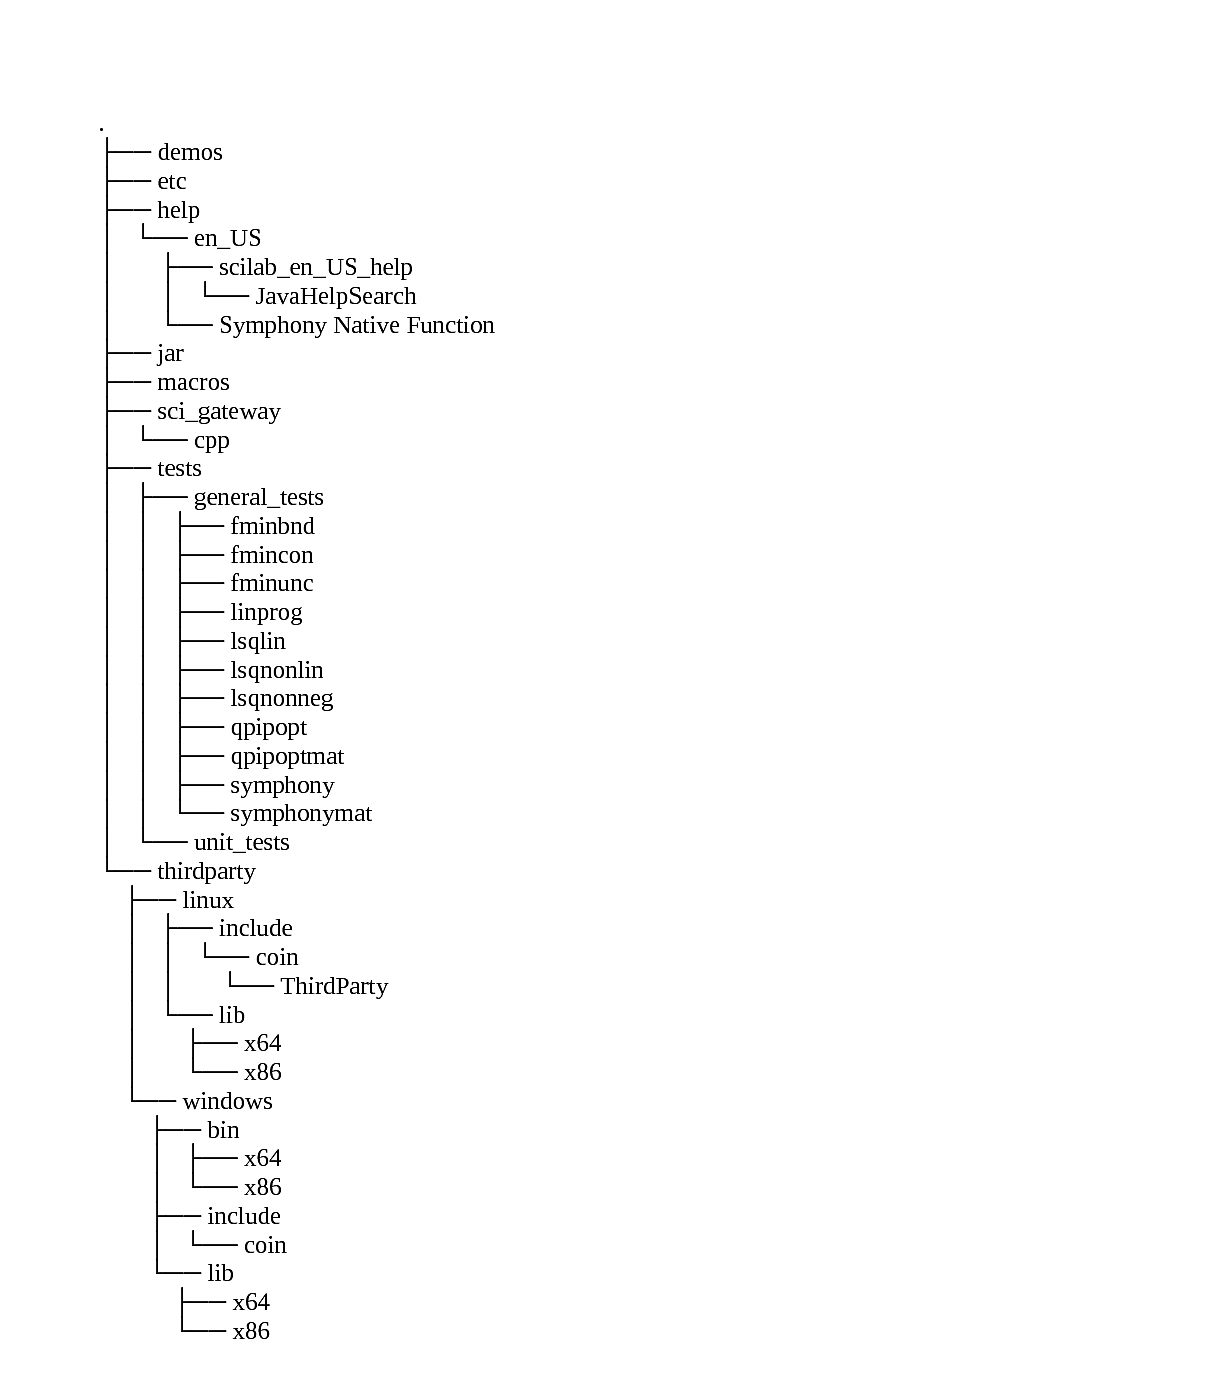
\includegraphics[width=\linewidth]{tree.jpg}
  \caption{FOT folder structure tree}
  \label{fig:Scilab2}
\end{figure}

Some of the important directories are :
\begin{enumerate}
	\item macros : Contains the scilab function files containing the functions that are to be called form Scilab and their respective builder files.
	\item sci\_gateway : Contains gateway files which are to be called from the thirdparty directory
	\item thirdparty : Contains the header files and dynamic linking libraries(shared libraries) of the toolbox classified by OS and architecture
	\item etc : Contains the files needed at the time of building the toolbox
	\item help : Contains the required help files for the toolbox
	\item tests : Contains the test files for the toolbox  
	\item demo : Contains demo files for the toolbox
\end{enumerate}

\chapter{Builder files}
\label{chap:Build}
\section{Introduction}
A builder file is a file used to build the toolbox. It creates binaries of the toolbox that is loaded into Scilab memory. Most of the directories mentioned in the previous chapter has their own builder files. The general file name of builder files are builder*.sce where * is replaced by a string.
\section{builder.sce}
The following is the main FOT builder.sce file which is located at the root directory:
\begin{lstlisting}[language=Scilab]
lines(0);
try
 getversion('scilab');
catch
 error(gettext('Scilab 5.0 or more is required.'));
end;
// ====================================================================
if ~with_module("development_tools") then
  error(msprintf(gettext("%s module not installed."),"development_tools"));
end
// ====================================================================
TOOLBOX_NAME = "FOSSEE_Optimization_Toolbox";
TOOLBOX_TITLE = "FOSSEE Optimization Toolbox";
// ====================================================================
toolbox_dir = get_absolute_file_path("builder.sce");
tbx_builder_macros(toolbox_dir);
tbx_builder_gateway(toolbox_dir);
tbx_builder_help(toolbox_dir);
tbx_build_loader(TOOLBOX_NAME, toolbox_dir);
tbx_build_cleaner(TOOLBOX_NAME, toolbox_dir);
clear toolbox_dir TOOLBOX_NAME TOOLBOX_TITLE;
\end{lstlisting}
\lstinline|lines(0)| disables vertical paging of the display.
The try-catch condition exits the builder if the required Scilab version is not available. The if loop following that checks if the development\_tool module is present. Generally, it should be present with your default Scilab installation. 
The following lines assign name and title, gets the path of the builder file and executes the other builder files which compiles the required directories with respective commands. It also builds a loader.sce which is used to load the binary files into Scilab memory and a cleaner.sce file to remove binary files.
\section{buildmacros.sce}
The buildmacros.sce file is located in macros directory. It compiles the scilab macro files which are scilab function files. The following is the content of the buildmacros.sce file:
\begin{lstlisting}[language=Scilab]
tbx_build_macros("FOSSEE_Optimization_Toolbox", 
							get_absolute_file_path("buildmacros.sce"));
clear tbx_build_macros;
\end{lstlisting}
\lstinline|tbx_build_macros| is the scilab function used to compile the macros file. The first argument is the toolbox name which is set in the main builder file and the second input is the path of the macros builder file. \lstinline|clear tbx_build_macros| clears the tbx\_build\_macros function from the scilab memory.
\section{builder\_gateway.sce}
builder\_gateway.sce file is used to run the compiles the builder files which are located in sub-directories.
\begin{lstlisting}[language=Scilab]

sci_gateway_dir = get_absolute_file_path('builder_gateway.sce');

tbx_builder_gateway_lang('cpp', sci_gateway_dir);
tbx_build_gateway_loader(['cpp'], sci_gateway_dir);

clear tbx_builder_gateway_lang tbx_build_gateway_loader;
clear sci_gateway_dir;
\end{lstlisting}
\lstinline|sci_gateway_dir| stores the path to the this file. \lstinline|tbx_builder_gateway_lang| runs the builder file in the respective sub-directories which in turn compiles the scripts. The first argument for this function is an array of languages which are to be compiled and the second argument is the path the builder\_gateway.sce file. The sub-directories have to be named in the name of the languages that the toolbox uses in these files. Scilab accepts C, C++ and FORTRAN as API languages.\\
\lstinline|tbx_build_gateway_loader(['cpp'], sci_gateway_dir);| generates the loader\_gateway script. The inputs are the same as \lstinline|tbx_builder_gateway_lang|.
\subsection{builder\_gateway\_cpp.sce}
\lstinline|builder_gateway_cpp.sce| file in \lstinline|root_dir/sci_gateway/cpp/| is the builder file for C++ files. The explanation for this file can be found in Section 4.6.4 of Michaël Baudin's article mentioned in \autoref{chap:Struct}.
\section{builder\_help.sce}
builder\_help.sce file is used to compile the help files which are located in directories, the names of which are the locales. locales are parameters which refers to the user's languages. The FOT uses en\_US locale and hence only has one sub-directory in the help directory.
\begin{lstlisting}[language=Scilab]
mode(-1)
lines(0)

toolbox_title = "FOSSEE_Optimization_Toolbox"

help_dir = get_absolute_file_path('builder_help.sce');

tbx_builder_help_lang("en_US", help_dir);

clear toolbox_title;
\end{lstlisting}
\lstinline|mode(-1)| executes the builder\_help.sce file silently. \lstinline|tbx_builder_help_lang| is used to build the help files which are located in the en\_US directory.
\chapter{etc directory}
\label{chap:etc}
\section{Introduction}
etc directory contains the initialization and finalization script of the toolbox which are run at the beginning and termination of the toolbox. They are executed while executing the loader and unloader files.
\section{FOSSEE\_Optimization\_Toolbox.start}
The name of the initialization script for a toolbox is the name of the toolbox followed by ".start". In our case, the name of the file is "FOSSEE\_Optimization\_Toolbox.start". The code for the same is given in Appendix \autoref{sec:FOSSEEStart}.

The FOSSEE\_Optimization\_Toolbox.start file is executed when we run the loader. It's purpose includes :
\begin{enumerate}
\item Load function libraries from macros directory.
\item Load gateway and shared libraries form sci\_gateway and thirdparty directory.
\item Load help from help directory.
\item Load demos from demos directory.
\end{enumerate}
\section{FOSSEE\_Optimization\_Toolbox.quit}
The name of the finalization script for a toolbox is the name of the toolbox followed by ".quit". In our case, the name of the file is "FOSSEE\_Optimization\_Toolbox.quit". The code for the same is given in \autoref{sec:FOSSEEquit}.

The FOSSEE\_Optimization\_Toolbox.quit file is executed when we run the loader. It's purpose includes :
\begin{enumerate}
\item Unlink the toolbox libraries.
\item Remove any preferences that was set by the toolbox.
\end{enumerate}

\chapter{macros directory}
\label{chap:macro}
\section{Introduction}
Macros folder contains scilab function files(*.sci). Files with extensions other than sci will not be compiled when the builder is run. Scilab macros can be:
\begin{enumerate}
\item A Scilab function file which returns the result after computation.
\item A Scilab function which calls a C, C++ or FORTRAN code.
\item A Scilab function which calls a binary library.
\end{enumerate}
In FOT, the macros files are of second kind which calls a C++ file. They should have the same file name as that of function inside. Except the licence information and some information's in comments ,the whole code and the help texts in comments are inside the function. 
\section{Outline of a macros file}
The general outline of most of macros files in FOT is as follows:
\begin{enumerate}
\item Help page comments
\item Input retrieval
\item Error checks
\item Input modifications
\item Call to the C++ library
\item Output retrieval,checks and modifications
\end{enumerate}
Lets take each of these steps and go through \lstinline|ROOT_DIR/macros/fmincon.sci| file to analyze it. The function is declared with \lstinline|function [xopt,fopt,exitflag,output,lambda,gradient,hessian] = fmincon (varargin)| where \lstinline|varargin| helps facilitates the input argument which can be a variable. It is a list with the input variables.
\subsection{Commented Help page}
The function declaration is immediately followed by the help documentation comments which is explained in detail in \autoref{chap:Help}.
\subsection{Input retrieval}
The inputs from the Scilab execution is parsed here using \lstinline|varargin| function. 
\begin{lstlisting}
[lhs , rhs] = argn();

//To check the number of arguments given by the user
if ( rhs<4 | rhs>10 ) then
	errmsg = msprintf(gettext("%s: Unexpected number of input arguments : %d provided while it should be 4,6,8,9,10"), "fmincon", rhs);
	error(errmsg)
end

if (rhs==5 | rhs==7) then
errmsg = msprintf(gettext("%s: Unexpected number of input arguments : %d provided while it should be 4,6,8,9,10s"), "fmincon", rhs);
error(errmsg)
end

//Storing the Input Parameters  
fun    	 = varargin(1);
x0   	 = varargin(2);
A    	 = varargin(3);
b    	 = varargin(4);
Aeq  	 = [];
beq  	 = [];
lb       = [];
ub       = [];
nlc      = [];

if (rhs>4) then
	Aeq  	 = varargin(5);
	beq  	 = varargin(6);
end

if (rhs>6) then
	lb       = varargin(7);
	ub       = varargin(8);
end

if (rhs>8) then
	nlc      = varargin(9);
end
\end{lstlisting}
\lstinline|argn| function returns the number of lhs and rhs arguments in the call. The subsequent \lstinline|if| conditions eliminate the possibility of unplanned inputs. \lstinline|varargin| being a list is parsed to extract the respective inputs.
\subsection{Error checks}
The code for Error checks is not shown here. It starts from the end of Input retrieval and goes on till the declaration of \lstinline|fGrad1| function. These error checks can be :
\begin{enumerate}
\item Checking the type of the variable passed. The \lstinline|Checktype.sci| file in the macros directory assists in this process.
\item Dimension checks in case of a real number,lists or Matrix.
\item Dependency checks. For example, if input A is empty, then input b should also be empty and vice versa. 
\item Initialization checks in case of a function to check if the current value is feasible for the function.
\item Double checks, to affirm the credibility of user provided values.
\item Content check, to check if the content of a variable is valid. For example, lower bound,lb cannot take infinity.
\item Input modification checks, if the given input has to be modified to get the actual input. For example, if an input taking row vector is given a column vector.
\end{enumerate}
\subsection{Input modifications}
The input modification for \lstinline|fmincon.sci| includes the functions \lstinline|fGrad1|,\lstinline|lHess1| and \lstinline|addcGrad1|. Some of the inputs are also modified in the above error checking process. In these modifications, the inputs are modified to suit to the specifications of the solver libraries.
\subsection{Call to the C++ library}
Following is the code to call the C++ library.
\begin{lstlisting}
//Creating a Dummy Variable for IPopt use
empty=[0];

//Calling the Ipopt function for solving the above problem
[xopt,fopt,status,iter,cpu,obj_eval,dual,lambda1,zl,zu,gradient,hessian1] = solveminconp(f,A,b,Aeq,beq,lb,ub,no_nlc,no_nlic,addnlc1,fGrad1,lHess1,addcGrad1,x0,options,empty)	
\end{lstlisting}
The empty dummy variable is provided to aid in retrieving functions in using \lstinline|scilab_call| API function of Scilab. We will discuss about it  in the coming sections.
\subsection{Output retrieval,checks and modifications}
The subsequent lines after calling the solver library are to manage output and pass it back to Scilab which are self-explanatory.
\chapter{sci\_gateway files}
\label{chap:gateway}
\section{Introduction}
The gateway files as the name suggests, acts as a gateway between Scilab and C++. The inputs from Scilab are not compatible with other languages and hence Scilab provides an array of API functions to accomplish this. sci\_gateway files generally are used to get input form Scilab ,pass it to the respective library, retrieve the results and pass the results back to Scilab. 

\section{Basic Scilab API Functions} 
The Scilab 6 API to pass and return values from C and C++ has been a major improvement over the previous versions of Scilab. In the context of the FOSSEE Optimization Toolbox, it reduces the dependence on the sci\_iofunc file. 

The main purpose of sci\_ iofunc file was to management input and output for FOT. It made the main code less cumbersome. However, since the advent of the new API, a lot of the advantages offered by sci\_iofunc are rendered moot. 


A list of API functions provided by Scilab can be found at this \urlthis{https://help.scilab.org/docs/6.0.2/en\_US/api\_scilab.html}{link}.These API functions are used in the interfaces directly, instead of relying on \lstinline|root_dir/sci_gateway/cpp/sci_iofunc.cpp| as we did in previous versions.

\section{Outline of a sci\_gateway file}
The general outline of a sci\_gateway file are as follows :
\begin{enumerate}
\item Variable initialization
\item Input retrieval
\item Input modifications, if any
\item Calling the library
\item Output management
\item Returning output to Scilab
\end{enumerate}
It is categorized so to help developers get an overall view of the functions. Many of the files don't have clear cut difference between two of the above said outline. We will go through this section with the help of \lstinline|root_dir/sci_gateway/cpp/cpp_intfmincon.cpp| file.
\subsection{Variable initialization}
Variable declarations are not just restricted to variables, but namespace declarations as well.
\begin{lstlisting}[language=C]
using namespace Ipopt;

if (nin !=13)  //Checking the input arguments
{
	Scierror(999, "%s: Wrong number of input arguments: %d expected.\n", fname, 13);
        	return STATUS_ERROR; 
}
	
if (nout !=3) //Checking the output arguments

{
	Scierror(999, "%s: Wrong number of output argument(s): %d expected.\n", fname, 3);
		return 1;
}



//Function pointers, input matrix(Starting point) pointer, flag variable 
double *x0ptr=NULL, *lbptr=NULL, *ubptr=NULL,*Aptr=NULL, *bptr=NULL, *Aeqptr=NULL, *beqptr=NULL;
double nonlinCon=0,nonlinIneqCon=0;
    

	// Input arguments
double *cpu_time=NULL,*max_iter=NULL;
static unsigned int nVars = 0,nCons = 0;
unsigned int temp1 = 0,temp2 = 0, iret = 0;
int x0_rows=0, x0_cols=0, lb_rows=0, lb_cols=0, ub_rows=0, ub_cols=0, A_rows=0, A_cols=0, b_rows=0, b_cols=0, Aeq_rows=0, Aeq_cols=0, beq_rows=0, beq_cols=0;

// Output arguments	
double  ObjVal=0,iteration=0,cpuTime=0,fobj_eval=0;
double dual_inf, constr_viol, complementarity, kkt_error;
const double *fX = NULL, *fGrad =  NULL;
const double *fHess =  NULL;
const double *fLambda = NULL;
const double *fZl=NULL;
const double *fZu=NULL;
int rstatus = 0;
int int_fobj_eval, int_constr_eval, int_fobj_grad_eval, int_constr_jac_eval, int_hess_eval;
\end{lstlisting}
\lstinline|nin| and \lstinline|nout| are Scilab API variables which check the inputs and outputs of the Scilab call.
\subsection{Input retrieval}
The following lines code below of \lstinline|sci_ipoptfmincon.cpp| retrieves the input from Scilab into C++. 
\begin{lstlisting}[language=C]
if (scilab_isDouble(env, in[5]) == 0 || scilab_isMatrix2d(env, in[5]) == 0)
	{
		Scierror(999, "%s: Wrong type for input argument #%d: A double matrix expected.\n", fname, 6);
		return 1;
	}
	
	scilab_getDoubleArray(env, in[5], &x0);
	int size1 = scilab_getDim2d(env, in[5], &x0_rows, &x0_cols);

	
	if (scilab_isDouble(env, in[6]) == 0 || scilab_isMatrix2d(env, in[6]) == 0)
	{
		Scierror(999, "%s: Wrong type for input argument #%d: A double matrix expected.\n", fname, 7);
		return 1;
	}
	
	scilab_getDoubleArray(env, in[6], &lb);

	

	if (scilab_isDouble(env, in[7]) == 0 || scilab_isMatrix2d(env, in[7]) == 0)
	{
		Scierror(999, "%s: Wrong type for input argument #%d: A double matrix expected.\n", fname, 8);
		return 1;
	}
	
	scilab_getDoubleArray(env, in[7], &ub);

	if (scilab_isDouble(env, in[8]) == 0 || scilab_isMatrix2d(env, in[8]) == 0)
	{
		Scierror(999, "%s: Wrong type for input argument #%d: A double matrix expected.\n", fname, 9);
		return 1;
	}
	
	scilab_getDoubleArray(env, in[8], &conLb);
	size1 = scilab_getDim2d(env, in[8], &nCons, &nCons2);

	

	if (scilab_isDouble(env, in[9]) == 0 || scilab_isMatrix2d(env, in[9]) == 0)
	{
		Scierror(999, "%s: Wrong type for input argument #%d: A double matrix expected.\n", fname, 10);
		return 1;
	}
	
	scilab_getDoubleArray(env, in[9], &conUb);
	

	// Getting intcon
	if (scilab_isDouble(env, in[10]) == 0 || scilab_isMatrix2d(env, in[10]) == 0)
	{
		Scierror(999, "%s: Wrong type for input argument #%d: A double matrix expected.\n", fname, 11);
		return 1;
	}
	
	scilab_getDoubleArray(env, in[10], &intcon);
	size1 = scilab_getDim2d(env, in[10], &intconSize, &intconSize2);



	if (scilab_isDouble(env, in[12]) == 0 || scilab_isMatrix2d(env, in[12]) == 0)
	{
		Scierror(999, "%s: Wrong type for input argument #%d: A double matrix expected.\n", fname, 13);
		return 1;
	}
	
	scilab_getDoubleArray(env, in[12], &LC);


	

    //Initialization of parameters

	//Getting parameters
	if (scilab_isList(env, in[11]) == 0)
    {
        Scierror(999, "%s: Wrong type for input argument #%d: A list expected.\n", fname, 12);
        return 1;
    }

	scilabVar temp1 = scilab_getListItem( env, in[11], 1);
	scilabVar temp2 = scilab_getListItem( env, in[11], 3);
	scilabVar temp3 = scilab_getListItem( env, in[11], 5);
	scilabVar temp4 = scilab_getListItem( env, in[11], 7);
	scilabVar temp5 = scilab_getListItem( env, in[11], 9);

	double integertolerance=0, allowable_gap=0, maxnodes =0,  cpuTime=0, maxiter=0;

	scilab_getDouble(env, temp1, &integertolerance);
	scilab_getDouble(env, temp2, &maxnodes);
	scilab_getDouble(env, temp3, &cpuTime);
	scilab_getDouble(env, temp4, &allowable_gap);
	scilab_getDouble(env, temp5, &maxiter);


	int max_nodes = (int)maxnodes;
	int cpu_time = (int)cpuTime;
	int iterLim = (int)maxiter;

\end{lstlisting}
Each of \lstinline|if| conditions processes one of inputs from Scilab and saves the address to a pointer which was declared earlier. \lstinline|getFixedSizeDoubleMatrixInList| is used to retrieve the options which are passed as a list.
\subsubsection{scilab\_call function}
\lstinline|scilab_call| is a C++ API function for Scilab which helps in evaluating a Scilab function at the given input. It is of particular interest because of the way it interacts with the Scilab call. We will see about this function with an example from \lstinline|root_dir/sci_gateway/cpp/sci_minconNLP.cpp|. Before we move ahead, give a thought to the inputs of the API call :
\begin{lstlisting}
[xopt,fopt,status,iter,cpu,obj_eval,dual,lambda1,zl,zu,gradient,hessian1] = solveminconp(f,A,b,Aeq,beq,lb,ub,no_nlc,no_nlic,addnlc1,fGrad1,lHess1,addcGrad1,x0,options,empty)	
\end{lstlisting}
Notice that the first input \lstinline|f| is a function, and so are the 10\textsuperscript{th},11\textsuperscript{th},12\textsuperscript{th} and 13\textsuperscript{th} input which are \lstinline|addnlc1|, \lstinline|fGrad1|, \lstinline|lHess1| and \lstinline|addcGrad1| respectively. There last three real inputs in the end, i.e. \lstinline|x0|,\lstinline|options| and \lstinline|empty|,the dummy variable.

Now we return to the \lstinline|minconNLP::eval_h| function in \lstinline|root_dir/sci_gateway/cpp/sci_minconNLP.cpp|. If the values are null, the hessian, which is represented as a sparse matrix is given random values. Else, the hessian matrix from is  taken in from Scilab using the following code :
\begin{lstlisting}[language=C++]
double check;


const Number *xNew=x;

const Number *lambdaNew=lambda;
double objfac=obj_factor;

scilabVar* funcIn = (scilabVar*)malloc(sizeof(scilabVar) * (numVars_) * 1);
funcIn[0] = scilab_createDoubleMatrix2d(env_, 1, numVars_, 0);
scilab_setDoubleArray(env_, funcIn[0], x);
double t= 2;
funcIn[1] = scilab_createDouble(env_, objfac);
funcIn[2] = scilab_createDoubleMatrix2d(env_, 1, numConstr_, 0);

scilab_setDoubleArray(env_, funcIn[2], lambdaNew);

scilab_call(env_, L"lHess1", 3, funcIn, 2, out);
                               
		
double* resCh;

if (scilab_isDouble(env_, out[1]) == 0 || scilab_isScalar(env_, out[1]) == 0)
{
	Scierror(999, "Wrong type for input argument #%d: An int expected.\n", 2);
			return 1;
}
		

scilab_getDouble(env_, out[1], &check);
if (check==1)
{
	return true;
}	
else
{                           
	if (scilab_isDouble(env_, out[0]) == 0 || scilab_isMatrix2d(env_, out[0]) == 0)
	{
		Scierror(999, "Wrong type for input argument #%d: An int expected.\n", 2);
				return 1;
	}
	
	scilab_getDoubleArray(env_, out[0], &resCh);
			
	Index index=0;
	for (Index row=0;row < numVars_ ;++row)
	{
		for (Index col=0; col < numVars_; ++col)
		{
			values[index++]=resCh[numVars_*row+col];
		}
	}
}

Index index=0;
for (Index row=0;row < numVars_ ;++row)
{
	for (Index col=0; col <= row; ++col)	
	{
		finalHessian_[n*row+col]=values[index++];
	}
}

index=0;
for (Index col=0;col < numVars_ ;++col)
{
	for (Index row=0; row <= col; ++row)	
	{
		finalHessian_[n*row+col]=values[index++];
	}
}
		
}	
\end{lstlisting}
\lstinline|scilab_call| function sends back the evaluated value of the Scilab function at input. In order to use \lstinline|scilab_call|, we have to obtain the the inputs using Scilab API writing function like \lstinline|scilab_getDouble|. Then \lstinline|scilab_call| function is called and the outputs from Scilab functions are overwritten over the first position of input that you gave earlier.

In this case, the lHess1 function in \lstinline|fmincon.sci| has three inputs and two outputs. For the three inputs, the \lstinline|get*| functions are used, with their respective arguments. The dummy variable was exclusively declared for this function as the other functions only have two inputs. \lstinline|scilab_call| has as the first input the name of the scilabEnv variable and the second is the function name. The third and fith inputs of the function are the numbers of inputs and outputs respectively. The fourth and sixth inputs are the pointers to the input and output variables. Once the \lstinline|scilab_call| function is executed, the outputs are written to the scilabVar* variable specificied in the output. Hence, you can see that check and resCh are retrieved from out[1] and out[0] respectively.
\subsection{Input modifications}
In this file, only these two lines modify the input.
\begin{lstlisting}[language=C]
//Number of variables and constraints
nVars = x0_cols;
nCons = A_rows + Aeq_rows + nonlinCon;

SmartPtr<minconNLP> Prob = new minconNLP(nVars, nCons, x0ptr, Aptr, bptr, Aeqptr, beqptr, A_rows, A_cols, b_rows, b_cols, Aeq_rows, Aeq_cols, beq_rows, beq_cols, lbptr, ubptr, nonlinCon, nonlinIneqCon);
\end{lstlisting}
The newly assigned variables are generally the required inputs for the solver library. They are not assigned and passed on from Scilab to reduce the API function usage.

The smart pointer \lstinline|SmartPtr| is declared in the namespace Ipopt. Here we create a new instance of minconNLP method, which is defined in \lstinline|root_dir/sci_gateway/cpp/sci_minconNLP.cpp|. minconNLP method is used to pass to modify the inputs in a way favourable to the solver. It is inspired from hs071\_nlp.hpp in the MyExample directory in earlier versions of Ipopt. In the latest version of Ipopt, the file is \lstinline|Ipopt/Ipopt/tutorial/CodingExercise/Cpp/1-skeleton/TutorialCpp_nlp.hpp|
\subsection{Calling the library}
In case of \lstinline|fmincon|, Ipopt solver is called.
\begin{lstlisting}[language=C]
SmartPtr<IpoptApplication> app = IpoptApplicationFactory();

////////// Managing the parameters //////////

app->Options()->SetNumericValue("tol", 1e-6);
app->Options()->SetIntegerValue("max_iter", (int)*max_iter);
app->Options()->SetNumericValue("max_cpu_time", *cpu_time);
//	app->Options()->SetStringValue("hessian_approximation", "limited-memory");

///////// Initialize the IpoptApplication and process the options /////////
ApplicationReturnStatus status;
status = app->Initialize();
if (status != Solve_Succeeded) 
{
  	sciprint("\n*** Error during initialization!\n");
		return (int) status;
	 }
 
 // Ask Ipopt to solve the problem
 status = app->OptimizeTNLP((SmartPtr<TNLP>&)Prob);
\end{lstlisting}
A new instance of Ipopt instance is made in the first line. We are using the \lstinline|IpoptApplicationFactory| since this allows us to compile this with an Ipopt Windows DLL. The respective options are passed  in the following lines . Hessian approximation option is commented out as we calculate the hessian in the Scilab macro and is already initiated in the \lstinline|Prob| instance.\\
In the following lines, the Ipopt library is initialized with the options. If the initialization succeeds, \lstinline| app->OptimizeTNLP((SmartPtr<TNLP>&)Prob)| solves the problem with the given parameters
\subsection{Output management}
The following lines of code manages the output of the solver that has to passed back to Scilab.
\begin{lstlisting}[language=C]
//Get the solve statistics
 cpuTime = app->Statistics()->TotalCPUTime();
 app->Statistics()->NumberOfEvaluations(int_fobj_eval, int_constr_eval, int_fobj_grad_eval, int_constr_jac_eval, int_hess_eval);
 app->Statistics()->Infeasibilities(dual_inf, constr_viol, complementarity, kkt_error);
 rstatus = Prob->returnStatus();
 fobj_eval=(double)int_fobj_eval;
     
////////// Manage the output argument //////////

fX = Prob->getX();
fGrad = Prob->getGrad();
fHess = Prob->getHess();
fLambda = Prob->getLambda();
fZl = Prob->getZl();
fZu = Prob->getZu();
ObjVal = Prob->getObjVal();
iteration = (double)app->Statistics()->IterationCount();
\end{lstlisting}
The above code is self-explanatory. The solver statistics are extracted form \lstinline|app| and the problem statistics are extracted from \lstinline|Prob|.
\subsection{Returning output to Scilab}
These lines of code return the required outputs back to Scilab. They are similar to the Input retrieval functions and are self-explanatory.
\begin{lstlisting}[language=C]
out[0] = scilab_createDoubleMatrix2d(env, 1, nVars, 0);
	scilab_setDoubleArray(env, out[0], fX);

	out[1] = scilab_createDouble(env, ObjVal);

	out[2] = scilab_createDouble(env, rstatus);
	out[3] = scilab_createDouble(env, iteration);
	out[4] = scilab_createDouble(env, cpuTime);
	out[5] = scilab_createDouble(env, fobj_eval);
	
	out[6] = scilab_createDouble(env, dual_inf);

	out[7] = scilab_createDoubleMatrix2d(env, 1, nCons, 0);
	scilab_setDoubleArray(env, out[7], fLambda);
	
	out[8] = scilab_createDoubleMatrix2d(env, 1, nVars, 0);
	scilab_setDoubleArray(env, out[8], fZl);

	out[9] = scilab_createDoubleMatrix2d(env, 1, nVars, 0);
	scilab_setDoubleArray(env, out[9], fZu);

	out[10] = scilab_createDoubleMatrix2d(env, 1, nVars, 0);
	scilab_setDoubleArray(env, out[10], fGrad);

	out[11] = scilab_createDoubleMatrix2d(env, 1, nVars*nVars, 0);
	scilab_setDoubleArray(env, out[11], fHess);

\end{lstlisting}
\chapter{Solver Libraries}
\label{chap:lib}
\section{Introduction}
This chapter deals with the compilation of solver and other libraries that are needed in the toolbox. It explains elaborately the tools and libraries needed to be compiled and related information
\section{Prerequisites}
Before we go ahead with library compilations, we need to setup our environment. The instructions that proceeds are meant for Linux operating systems, specifically Debian OS. Windows User are advised to install Cygwin and take necessary steps where required.Execute the following command on the terminal to install the needed packages\\
\lstinline|$ sudo apt-get install git subversion build-essential gfortran|\\
\section{Compiling libraries}
FOSSEE Optimization toolbox directly uses the following libraries for their respective solving domains:
\begin{enumerate}
	\item CLP
	\item Symphony
	\item Ipopt
	\item Bonmin
	\item CBC
	\item ecos
\end{enumerate}
\noindent But since the dependent libraries of these solvers have gone ahead with many minor releases when compared to the one included in the respective solvers, it is recommended to replace the dependent libraries in the solver library with the latest version.Hence the list of the libraries other than the one given above are :
\begin{enumerate}
	\item CLP
	\item CGL
	\item OSI
	\item CoinUtils
\end{enumerate}
These libraries can be downloaded directly or by \urlthis{subversion.tigris.org/}{subversion} or git. The download information can be found at their respective websites.

We will be giving step-by-step instruction on compilation of the source code of all the libraries required. Many of the steps are same for most of the solvers.
\subsection{ecos}
ecos is  lightweight second order conic optimization solver which is written in C. In FOT, \lstinline|ecos| function uses the ecos library. The steps to download, modify and compile ecos source code are given below:
\begin{enumerate}
\item The ecos source code is hosted on github at this  \urlthis{https://github.com/embotech/ecos}{link}. Download using \lstinline|$ git clone https://github.com/embotech/ecos.git ECOS|.
\item Since there are function names conflicts between ecos and scilab, we have to change the names in ecos source code before we compile. This can be done by running the following commands.
\begin{lstlisting}[language=sh]
$ cd ECOS
$sed -ir 's/createSparseMatrix/EcosCreateSparseMatrix/g' *
\end{lstlisting}
\item Run the following command to compile ecos source code and generate shared library.
\begin{lstlisting}[language=sh]
$ make shared
\end{lstlisting}
\end{enumerate}
The shared libraries will be generated in \lstinline|ECOS| and the header files will be in \lstinline|ECOS/include| and \lstinline|ECOS/external|.

\subsection{CLP}
CLP or COIN-OR Linear Programming is an open-source LP solver written in C++. In FOT, \lstinline|linprog| uses CLP library.
The latest version of CLP can be downloaded from the following \urlthis{https://projects.coin-or.org/svn/Clp/releases/}{link}. CLP depends on three other COIN-OR projects, namely BuildTools,CoinUtils and OSI.
The steps to download, modify and compile CLP source code are given below:
\begin{enumerate}
	\item Download using \lstinline|$ svn co https://projects.coin-or.org/svn/Clp/releases/x.xx.xx CLP|.The x.xx.xx in the end of svn link should to be replaced with the respective version that is to be downloaded. Hence CLP will be downloaded into a directory called CLP.
	\item Run \lstinline|get.Lapack|, \lstinline|get.Mumps| and \lstinline|getBlas| in Lapack, Mumps and Blas subdirectory in the \lstinline|CLP/ThirdParty| from the terminal.\\
	\begin{lstlisting}[language=sh]
$ ./CLP/ThirdParty/Lapack/get.Lapack
$ ./CLP/ThirdParty/Blas/get.Blas
$ ./CLP/ThirdParty/Mumps/get.Mumps
	\end{lstlisting}
	\item The dependencies on which CLP depends on has to be replaced with the latest version of the same. They can be downloaded from the following \urlthis{https://projects.coin-or.org/svn/}{link}. Download them in the same directory where CLP is downloaded as they will be used by other solvers as well.\\
\begin{lstlisting}[language=sh]
$ svn co https://projects.coin-or.org/svn/BuildTools/releases/x.xx.xx BUILDTOOLS
$ svn co https://projects.coin-or.org/svn/CoinUtils/releases/y.yy.yy COINUTILS
$ svn co https://projects.coin-or.org/svn/OSI/releases/z.zz.zz OSI
\end{lstlisting}

	\item Move the current dependencies to another directory and replace it with the latest ones that was downloaded in the previous step. For example, for CoinUtils, move the \lstinline|CLP/CoinUtils| to \lstinline|CLP/Old.CoinUtils| and move \lstinline|CoinUtils/CoinUtils| to \lstinline|CLP/CoinUtils|.Please note that the new CoinUtils directory to be replaced is inside the main CoinUtils directory. The same is done for BuildTools and OSI as well.
	\begin{lstlisting}[language=sh]
$ mv CLP/BuildTools CLP/Old.BuildTools
$ mv BUILDTOOLS/BuildTools CLP/BuildTools
$ mv CLP/CoinUtils CLP/Old.CoinUtils
$ mv COINUTILS/CoinUtils CLP/CoinUtils
$ mv CLP/Osi CLP/Old.Osi
$ mv OSI/Osi CLP/Osi
	\end{lstlisting}
	\item Make a directory called \lstinline|build| and go into that directory. Run the \lstinline|configure| script followed by \lstinline|make| and \lstinline|make install|.
	\begin{lstlisting}[language=sh]
$ mkdir build
$ cd build
$ ../configure
$ make
$ make install
	\end{lstlisting}
	
\end{enumerate}
The shared libraries will be generated in \lstinline|CLP/build/lib| and the header files will be in \lstinline|CLP/build/include|.

\subsection{Symphony}
Symphony is yet another Linear Programming solver which is an open-source written in C++. In FOT, \lstinline|symphony| and \lstinline|symphonymat| uses Symphony.
The latest version of Symphony can be downloaded from the following \urlthis{https://projects.coin-or.org/svn/Symphony/releases/}{link}. Symphony depends the following COIN-OR projects :
\begin{enumerate}
\item CGL
\item CLP
\item CoinUtils
\item OSI
\item BuildTools
\end{enumerate}
The steps to download, modify and compile Symphony source code are given below:
\begin{enumerate}
	\item Download using \lstinline|$ svn co https://projects.coin-or.org/svn/Symphony/releases/x.xx.xx SYMPHONY|.The x.xx.xx in the end of svn link should to be replaced with the respective version that is to be downloaded. Hence Symphony will be downloaded into a directory called SYMPHONY.
	\item Run \lstinline|get.Lapack| and \lstinline|getBlas| in Lapack and Blas subdirectory in the \lstinline|Symphony/ThirdParty| from the terminal.\\
	\begin{lstlisting}[language=sh]	
$ ./SYMPHONY/ThirdParty/Lapack/get.Lapack
$ ./SYMPHONY/ThirdParty/Blas/get.Blas
	\end{lstlisting}
	\item The dependencies on which Symphony depends on has to be replaced with the latest version of the same. They can be downloaded from the following \urlthis{https://projects.coin-or.org/svn/}{link}. Download them in the same directory where Symphony is downloaded as they will be used by other solvers as well. Ignore the libraries which have been already downloaded.\\
\begin{lstlisting}[language=sh]
$ svn co https://projects.coin-or.org/svn/Cgl/releases/x.xx.xx CGL
$ svn co https://projects.coin-or.org/svn/Clp/releases/y.yy.yy CLP
$ svn co https://projects.coin-or.org/svn/CoinUtils/releases/z.zz.zz COINUTILS
$ svn co https://projects.coin-or.org/svn/OSI/releases/w.ww.ww OSI
$ svn co https://projects.coin-or.org/svn/BuildTools/releases/v.vv.vv BUILDTOOLS

\end{lstlisting}	
	\item Move the current dependencies to another directory and replace it with the latest ones that was downloaded in the previous step.
	\begin{lstlisting}[language=sh]
$ mv SYMPHONY/Cgl SYMPHONY/Old.Cgl
$ mv CGL/Cgl SYMPHONY/Cgl
$ mv SYMPHONY/Clp SYMPHONY/Old.Clp
$ mv CLP/Clp SYMPHONY/Clp
$ mv SYMPHONY/CoinUtils SYMPHONY/Old.CoinUtils
$ mv COINUTILS/CoinUtils SYMPHONY/CoinUtils
$ mv SYMPHONY/Osi SYMPHONY/Old.Osi
$ mv OSI/Osi SYMPHONY/Osi
$ mv SYMPHONY/BuildTools SYMPHONY/Old.BuildTools
$ mv OSI/BUILDTOOLS SYMPHONY/BuildTools
	\end{lstlisting}
	\item Make a directory called \lstinline|build| and go into that directory. Run the \lstinline|configure| script followed by \lstinline|make| and \lstinline|make install|.
	\begin{lstlisting}[language=sh]
$ mkdir build
$ cd build
$ ../configure
$ make
$ make install
	\end{lstlisting}
	
\end{enumerate}
The shared libraries will be generated in \lstinline|SYMPHONY/build/lib| and the header files will be in \lstinline|SYMPHONY/build/include|. 

\subsection{Ipopt}
Ipopt or Interior Point Optimizer is a non-linear programming optimization solver which is an open-source written in C++. In FOT, \lstinline|fminunc|, \lstinline|fminbnd|, \lstinline|fmincon|,\lstinline|fminimax|, \lstinline|fgoalattain|, \lstinline|lsqlin|, \lstinline|lsqnonlin|,\lstinline|lsqnonneg| and \lstinline|qpipopt| uses Ipopt.
The latest version of Ipopt can be downloaded from the following \urlthis{https://projects.coin-or.org/svn/Ipopt/releases/}{link}. Ipopt depends on only BuildTools.
The steps to download, modify and compile Ipopt source code are given below:
\begin{enumerate}
	\item Download using \lstinline|$ svn co https://projects.coin-or.org/svn/Ipopt/releases/x.xx.xx IPOPT|.The x.xx.xx in the end of svn link should to be replaced with the respective version that is to be downloaded. Hence Ipopt will be downloaded into a directory called IPOPT.
	\item Run \lstinline|get.Lapack|,\lstinline|get.Mumps| and \lstinline|getBlas| in Lapack, Mumps and Blas subdirectory in the \lstinline|IPOPT/ThirdParty| from the terminal.\\
	\begin{lstlisting}[language=sh]
$ ./IPOPT/ThirdParty/Lapack/get.Lapack
$ ./IPOPT/ThirdParty/Mumps/get.Mumps
$ ./IPOPT/ThirdParty/Blas/get.Blas
	\end{lstlisting}
	\item Make a directory called \lstinline|build| and go into that directory. Run the \lstinline|configure| script followed by \lstinline|make| and \lstinline|make install|.
	\begin{lstlisting}[language=sh]	
$ mkdir build
$ cd build
$ ../configure
$ make
$ make install
	\end{lstlisting}
	
\end{enumerate}
The shared libraries will be generated in \lstinline|IPOPT/build/lib| and the header files will be in \lstinline|IPOPT/build/include|.

\subsection{CBC}
CBC is yet another Linear Programming solver which is an open-source written in C++. In FOT, \lstinline|cbcintlinprog| and \lstinline|cbcmatrixlinprog| uses CBC.
The latest version of CBC can be downloaded from the following \urlthis{https://projects.coin-or.org/svn/Cbc/releases/}{link}. CBC depends the following COIN-OR projects :
\begin{enumerate}
\item CGL
\item CLP
\item CoinUtils
\item OSI
\item BuildTools
\end{enumerate}
The steps to download, modify and compile CBC source code are given below:
\begin{enumerate}
	\item Download using \lstinline|$ svn co https://projects.coin-or.org/svn/Cbc/releases/x.xx.xx CBC|.The x.xx.xx in the end of svn link should to be replaced with the respective version that is to be downloaded. Hence Cbc will be downloaded into a directory called SYMPHONY.
	\item Run \lstinline|get.Lapack|, \lstinline|get.Mumps| and \lstinline|getBlas| in Lapack and Blas subdirectory in the \lstinline|CBC/ThirdParty| from the terminal.\\
	\begin{lstlisting}[language=sh]	
$ ./CBC/ThirdParty/Lapack/get.Lapack
$ ./CBC/ThirdParty/Mumps/get.Mumps
$ ./CBC/ThirdParty/Blas/get.Blas
	\end{lstlisting}
	\item The dependencies on which CBC depends on has to be replaced with the latest version of the same. They can be downloaded from the following \urlthis{https://projects.coin-or.org/svn/}{link}. Download them in the same directory where CBC is downloaded as they will be used by other solvers as well. Ignore the libraries which have been already downloaded.\\
\begin{lstlisting}[language=sh]
$ svn co https://projects.coin-or.org/svn/Cgl/releases/x.xx.xx CGL
$ svn co https://projects.coin-or.org/svn/Clp/releases/y.yy.yy CLP
$ svn co https://projects.coin-or.org/svn/CoinUtils/releases/z.zz.zz COINUTILS
$ svn co https://projects.coin-or.org/svn/OSI/releases/w.ww.ww OSI
$ svn co https://projects.coin-or.org/svn/BuildTools/releases/w.ww.ww BUILDTOOLS
\end{lstlisting}	
	\item Move the current dependencies to another directory and replace it with the latest ones that was downloaded in the previous step.
	\begin{lstlisting}[language=sh]
$ mv CBC/Cgl CBC/Old.Cgl
$ mv CGL/Cgl CBC/Cgl
$ mv CBC/Clp CBC/Old.Clp
$ mv CLP/Clp CBC/Clp
$ mv CBC/CoinUtils CBC/Old.CoinUtils
$ mv COINUTILS/CoinUtils CBC/CoinUtils
$ mv CBC/Osi CBC/Old.Osi
$ mv OSI/Osi CBC/Osi
$ mv CBC/BuildTools CBC/Old.BuildTools
$ mv BUILDTOOLS/BuildTools CBC/BuildTools
	\end{lstlisting}
	\item Make a directory called \lstinline|build| and go into that directory. Run the \lstinline|configure| script followed by \lstinline|make| and \lstinline|make install|.
	\begin{lstlisting}[language=sh]	
$ mkdir build
$ cd build
$ ../configure
$ make
$ make install
	\end{lstlisting}
	
\end{enumerate}
The shared libraries will be generated in \lstinline|CBC/build/lib| and the header files will be in \lstinline|CBC/build/include|. 

\subsection{Bonmin}
Bonmin is yet another Linear Programming solver which is an open-source written in C++. In FOT, \lstinline|intfminunc|, \lstinline|intfminbnd|, \lstinline|intfmincon| and \lstinline|intfminimax| uses Bonmin.
The latest version of Bonmin can be downloaded from the following \urlthis{https://projects.coin-or.org/svn/Bonmin/releases/}{link}. Bonmin depends the following COIN-OR projects :
\begin{enumerate}
\item CGL
\item CLP
\item CoinUtils
\item OSI
\item BuildTools
\item Ipopt
\item CBC
\end{enumerate}
The steps to download, modify and compile CBC source code are given below:
\begin{enumerate}
	\item Download using \lstinline|$ svn co https://projects.coin-or.org/svn/Bonmin/releases/x.xx.xx BONMIN|.The x.xx.xx in the end of svn link should to be replaced with the respective version that is to be downloaded. Hence Cbc will be downloaded into a directory called BONMIN.
	\item Run \lstinline|get.Lapack|, \lstinline|get.Mumps| and \lstinline|getBlas| in Lapack and Blas subdirectory in the \lstinline|BONMIN/ThirdParty| from the terminal.\\
	\begin{lstlisting}[language=sh]
$ ./BONMIN/ThirdParty/Lapack/get.Lapack
$ ./BONMIN/ThirdParty/Mumps/get.Mumps
$ ./BONMIN/ThirdParty/Blas/get.Blas
	\end{lstlisting}
	\item The dependencies on which CBC depends on has to be replaced with the latest version of the same. They can be downloaded from the following \urlthis{https://projects.coin-or.org/svn/}{link}. Download them in the same directory where CBC is downloaded as they will be used by other solvers as well. Ignore the libraries which have been already downloaded.\\
\begin{lstlisting}[language=sh]
$ svn co https://projects.coin-or.org/svn/Cgl/releases/x.xx.xx CGL
$ svn co https://projects.coin-or.org/svn/Clp/releases/y.yy.yy CLP
$ svn co https://projects.coin-or.org/svn/CoinUtils/releases/z.zz.zz COINUTILS
$ svn co https://projects.coin-or.org/svn/OSI/releases/w.ww.ww OSI
$ svn co https://projects.coin-or.org/svn/Ipopt/releases/w.ww.ww IPOPT
$ svn co https://projects.coin-or.org/svn/Cbc/releases/w.ww.ww CBC
\end{lstlisting}	
	\item Move the current dependencies to another directory and replace it with the latest ones that was downloaded in the previous step.
	\begin{lstlisting}[language=sh]
$ mv BONMIN/Cgl BONMIN/Old.Cgl
$ mv CGL/Cgl BONMIN/Cgl
$ mv BONMIN/Clp BONMIN/Old.Clp
$ mv CLP/Clp BONMIN/Clp
$ mv BONMIN/CoinUtils BONMIN/Old.CoinUtils
$ mv COINUTILS/CoinUtils BONMIN/CoinUtils
$ mv BONMIN/Osi BONMIN/Old.Osi
$ mv OSI/Osi BONMIN/Osi
$ mv BONMIN/BuildTools BONMIN/Old.BuildTools
$ mv BUILDTOOLS/BuildTools BONMIN/BuildTools
$ mv BONMIN/Ipopt BONMIN/Old.Ipopt
$ mv IPOPT/Ipopt BONMIN/Ipopt
$ mv BONMIN/Cbc BONMIN/Old.Cbc
$ mv CBC/Cbc BONMIN/Cbc
	\end{lstlisting}
	\item Make a directory called \lstinline|build| and go into that directory. Run the \lstinline|configure| script followed by \lstinline|make| and \lstinline|make install|.
	\begin{lstlisting}[language=sh]
$ mkdir build
$ cd build
$ ../configure
$ make
$ make install
	\end{lstlisting}
	
\end{enumerate}
The shared libraries will be generated in \lstinline|BONMIN/build/lib| and the header files will be in \lstinline|BONMIN/build/include|. 

\section{Shared libraries}
Files having extension \lstinline|*.so*| are called shared or dynamic libraries in Linux. In case of windows they are \lstinline|*.dll| and \lstinline|*.lib|. In FOT, the shared libraries have to be compiled for only windows and linux. it has to compiled for different architectures(x64 and x32) as well. The windows dlls are kept in \lstinline|ROOT_DIR/thirdparty/windows/bin/| and \lstinline|ROOT_DIR/thirdparty/windows/lib/|. Both of these directories have \lstinline|x64| and \lstinline|x32| directories. The Linux shared libraries are in  \lstinline|ROOT_DIR/thirdparty/linux/lib/| which again has \lstinline|x64| and \lstinline|x32| directories. Copy all the shared libraries having *.so* extension generated in the previous section into the respective architecture directory.
\section{Header files}
Files having extension \lstinline|*.h| or \lstinline|*.hpp| are called header files. The windows header files are kept in \lstinline|ROOT_DIR/thirdparty/windows/include/|. The linux shared libraries are in  \lstinline|ROOT_DIR/thirdparty/linux/include/|. Copy all the header files generated in the previous section into the these directory.

\chapter{Help Files}
\label{chap:Help}
	\section{Introduction}
	The FOSSEE Optimization Toolbox has an extensive help section that covers all of the functions that the toolbox currently consists of. This chapter will explain the basic structure of a standard help document, the methods to make it, and the preferred style to be used while making it. The appendix contains a short tutorial on how to create a simple help document for a toolbox function.
	\section{Basic help document structure}
	The sections included in a standard help document are:
	\begin{itemize}
	\item Calling Sequence: Describe the calling sequence of the function, mentioning all possible variations of inputs, and outputs.
	\item Input Parameters: Describe each of the Input Parameters of the function.
	\item Outputs: Describe each of the Outputs of the function.
	\item Description: Mathematical description of the type of problem being solved. 
	\item Options: Detail the solver options available to the user.
	\item Misc.: Describing the exitflags, the output data structure, and other outputs of the function.
	\item Examples: Provide examples demonstrating the usage of the function, and cases where a solution is not possible. 
	\item Authors: Name the authors.		
	\end{itemize}
	To get a better idea of the structure, see the structure of a help document currently being used.
	
		\urlthis{http://www.scilab.in/scilab-toolbox-help-files/fmincon.php}{fmincon}

	%	\begin{tcolorbox}[breakable,notitle,boxrule=0pt,colback=blue!20,colframe=blue!20]
	%		\textsc{NOTE}\\
	%		Something that is odd, not normal can be added in these boxes
	%	\end{tcolorbox}
	%	
	%	\verb|$ sudo apt-get install git| %use \verb for inline codes
	%
	%	\begin{lstlisting} %use lstlisting for longer codes
	%	gfhgfhf
	%	\end{lstlisting} 
	\section{Methods of writing help documents}
	In this section, we touch upon the methods via which you can write the help documents.
	\subsection{Using help\_from\_sci}
	Scilab provides means to generate a help document for a macro directly from comments made in it. After defining the function, the user can write the documentation in english, and use the function \lstinline|help_from_sci| to compile the help document from it. To generate a basic function template with a basic documentation skeleton, use \lstinline|help_from_sci(funname,helpdir)|.
		\subsubsection{Sections available in help\_from\_sci}
	The following sections are available directly while generating documentation \lstinline|via help_from_sci|. 
	\begin{itemize}
	\item Calling Sequence
	\item Parameters
	\item Description
	\item Examples
	\item Authors
	\end{itemize}
	\subsection{Directly via XML}
	This is akin to writing a simple webpage and provides the developer with all the freedom that they have while writing a webpage. The style sheet is already provided within the toolbox, so that won't prove to be a problem. This method, however, will prove to be time consuming because the developer will have to write everything from scratch, and that might prove to be time consuming.
	
	An easier way to go about this might be to generate a basic help page skeleton using help\_from\_sci and then modifying the generated XML file in help/en\_US as needed to make a help document according to the developer's requirements. 
	
	\section{Style Preferences}
	\begin{itemize}
	\item Calling Sequence: The calling sequence is to be enclosed in <synopsis> tags.
	\item The Input parameters and the outputs will be part of a single refsection.
	\item The problem description, options, and misc. details will be enclosed in a single refsection. \LaTeX \  should be used to provide the mathematical description.
	\item Examples: \LaTeX \ should be used to specify the problem being solved. The code snippets are to be enclosed in a <programlisting> tag. Each example will be enclosed in a separate refsection.
	\end{itemize}
	
	\subsection{Using \LaTeX}
	
	\lstinline|<latex>| tags have been provided for typesetting mathematical equations. It is advised that it be used within \lstinline|<para>| tags. Basic \LaTeX \  functionality has been included in this, but no packages are to be used. Equations can be aligned using \lstinline|{eqnarray}|. There is no need to use standard \LaTeX \  commands to begin documents. The developer can simply enter the \lstinline|<latex>| tags and start working. 
	
	\section{Additional Notes}
	The following observations were made while developing the current batch of help documents and the developer is advised to be familiar with them.
	\subsection{Problems faced while using \LaTeX}
	\begin{itemize}
	\item The developer will face some minor issues while using \LaTeX \ in the documentation.  The first and most obvious one will be that in some help files, they will run into an error if they begin a line with an ampersand. This error won't show up on the log, but will prevent the chunk of \LaTeX \ information from rendering in the document. Currently, we do not know what is causing this error, but to work around it, the developer can add, for example, a \lstinline|\hspace{1pt}| before the ampersand.
	
	\item Another thing that the developer will face in the same files that will have the aforementioned ampersand issue is that they will not be able to use multiple ampersands next to each other. The developer is advised to avoid doing so, and use \lstinline|\qquad| or \lstinline|hspace|.
	
	\item The developer will notice that the term 'some files' has been used. This is because the issue currently affects less than half the files. It specifically affects those files that are at the end of the sorting system, which currently is the alphabetical order.
	\end{itemize}

\begin{appendices}
\chapter{Codes}
\label{chap:Codes}
\section{FOSSEE\_Optimization\_Toolbox.start}
\label{sec:FOSSEEStart}
\lstset{language=Scilab, 
numbers=left, 
frame=single, 
captionpos=t,
showstringspaces=false,
breaklines=true,
breakatwhitespace=false,
tabsize=3
}
\begin{lstlisting}[language=Scilab]
mprintf("Start FOSSEE Optimization Toolbox\n");

[a, opt] = getversion();
Version = opt(2);

etc_tlbx  = get_absolute_file_path("FOSSEE_Optimization_Toolbox.start");
etc_tlbx  = getshortpathname(etc_tlbx);
root_tlbx = strncpy( etc_tlbx, length(etc_tlbx)-length("\etc\") );

//Load  functions library

mprintf("\tLoad macros\n");
if (getos()=="Windows") then
    pathmacros = pathconvert( root_tlbx ) + "macros_win" + filesep();
    symphony_lib = lib(pathmacros);
    clear pathmacros;
else
    pathmacros = pathconvert( root_tlbx ) + "macros" + filesep();
    symphony_lib = lib(pathmacros);
    clear pathmacros;
end

// load gateways

mprintf("\tLoad gateways\n");
[a, opt] = getversion();
Version = opt(2);
ilib_verbose(0);
if getos()=="Windows" then
    lib_path = root_tlbx + "/thirdparty/windows/bin/" + Version;
    link(lib_path+filesep()+"IpOptFSS.dll");
    link(lib_path+filesep()+"IpOpt-vc10.dll");
else
    lib_path = root_tlbx + "/thirdparty/linux/lib/" + Version;
    link(lib_path + "/libCoinUtils.so");
    link(lib_path + "/libcoinblas.so");
    link(lib_path + "/libcoinlapack.so");
    link(lib_path + "/libcoinmumps.so");
    link(lib_path + '/libCbc.so');
    link(lib_path + "/libClp.so");
    link(lib_path + "/libClpSolver.so");
    link(lib_path + "/libOsi.so");
    link(lib_path + "/libOsiCommonTests.so");
    link(lib_path + "/libOsiClp.so");
    link(lib_path + "/libCgl.so");
    link(lib_path + "/libSym.so");
    link(lib_path + "/libOsiSym.so");  
    link(lib_path + "/libipopt.so");
    link(lib_path + '/libbonmin.so');
    link(lib_path + "/libecos.so");
end
exec(pathconvert(root_tlbx + filesep() + "sci_gateway" + filesep() + "loader_gateway.sce",%f));

// Load and add help chapter

if ( %t ) then
if or(getscilabmode() == ["NW";"STD"]) then
        mprintf("\tLoad help\n");
        path_addchapter = pathconvert(root_tlbx+"/jar");
        if ( isdir(path_addchapter) <> [] ) then
                add_help_chapter("FOSSEE_Optimization_Toolbox", path_addchapter, %F);
                clear add_help_chapter;
        end
        clear path_addchapter;
end
end

// add demos

if ( %t ) then
if or(getscilabmode() == ["NW";"STD"]) then
    mprintf("\tLoad demos\n");
    pathdemos = pathconvert(root_tlbx+"/demos/sci_FOSSEE_Optimization_Toolbox.dem.gateway.sce",%f,%t);
    add_demo("FOSSEE_Optimization_Toolbox",pathdemos);
    clear pathdemos ;
end
end

clear etc_tlbx root_tlbx Version a opt lib_path;
\end{lstlisting}


\section{FOSSEE\_Optimization\_Toolbox.quit}
\label{sec:FOSSEEquit}
\begin{lstlisting}[language=Scilab]
function quitModule()

    etc_tlbx  = get_absolute_file_path("FOSSEE_Optimization_Toolbox.quit");
    etc_tlbx  = getshortpathname(etc_tlbx);
    root_tlbx = strncpy( etc_tlbx, length(etc_tlbx)-length("\etc\") );

    //unlink libraries
    [bOK, ilib] = c_link('FOSSEE_Optimization_Toolbox');
    if bOK then
        ulink(ilib);
    end

    // Remove Preferences GUI
    if getscilabmode() == "STD" then
    removeModulePreferences(root_tlbx);
    end
	ulink();
endfunction

quitModule();

clear quitModule;
\end{lstlisting}
\chapter{Tutorial}
\label{chap:Tutorials}
\lstset{
numbers=none, 
captionpos=b,
showstringspaces=false,
breaklines=true,
breakatwhitespace=false,
tabsize=3
}
\section{Toolbox Tutorial}
\section{Help Tutorial}
	\subsection{Introduction}
	Here we see how to go about making a basic help document for a function in the FOT. Both methods of doing so have been illustrated below:
	\subsection{Using help\_from\_sci}	
	\begin{itemize}
	\item Use \lstinline|help_from_sci()| to generate a basic skeleton for the documentation, along with the function. Save it as \lstinline|funname.sci|
	\item Write the function, and the documentation as discussed in the chapter on help documents. 
	\item Enter the command \lstinline|help_from_sci(funname,helpdir)| to generate the help document from the function.
	\item Once done, open scilab and build the FOT. You can see the help document on using the help command.
	\end{itemize}
	\subsubsection{Example}
	\begin{lstlisting}[language=Scilab]
	--> help_from_sci() 
	\end{lstlisting}
	This will generate a function template. We save the following function in the template, and modify the filename accordingly.
	\begin{lstlisting}[language=Scilab]
	function [y, z]=funname(a, b)
    	y=a+b,z=1;
    	endfunction
	\end{lstlisting}
	After modifying the documentation as necessary, we use the following command to generate a help document in the same directory.
	\begin{lstlisting}[language=Scilab]
	--> help_from_sci(funname,".")
	\end{lstlisting}
	
	\subsection{Modifying the XML}
	This method has its basis in the method described above, but here the developer has a lot more freedom. In this method, the developer can simply edit the XML file generated by the previous method, and implement a lot of their own ideas about the documentation.
	
	In this method, the developer should generate a basic XML file as displayed in the previous subsection. And then go on to make changes as needed. There isn't a lot to write here because this section depends largely on the developer's comfort with XML.
	
	To view the modifications made, simply rebuild the FOT once the modifications have been made, and use the help command to view them.
\chapter{Assignments}
\label{chap:Assgt}
%\section{Introduction}
\begin{enumerate}
\item Make a gateway file of a language of your choice that accepts two matrices and returns the
	\begin{enumerate}
		\item Sum of both matrices
		\item Difference of both matrices
		\item Multiplication of both matrices
		\item All the above three operations. Use a third input which specifies which operation is to be performed.
	\end{enumerate}
\item Go through the sourcecode of lp\_solve API given at this \urlthis{https://sourceforge.net/projects/lpsolve/files/lpsolve/5.5.2.5/lp\_solve\_5.5.2.5\\ \_scilab\_source.tar.gz/download}{link}. Understand the implementation and try to make a FOT implementation of the same similar to \lstinline|intlinprog|.
\item Create the same for \urlthis{https://github.com/ycollet/scilab-mip/tree/master/sciglpk}{GLPK}.
\end{enumerate}
\end{appendices}
\end{document}